\section{Experiments}

\subsection{Experimental Setup}

\paragraph{Dataset.}  
We pre-train on the autonomous driving dataset nuScenes~\cite{nuscenes} and the largest-scale 3D occupancy dataset OpenScene~\cite{openscene}, and fine-tune on nuScenes. Evaluation settings are the same as UniAD~\cite{uniad}. For detailed dataset descriptions, please refer to the Section~\ref{data} in the supplemental material..
%\vspace{-1em}
\paragraph{Pre-training.}
In alignment with BEVFormer~\cite{bevformer} and UniAD~\cite{uniad}, we employ ResNet101-DCN~\cite{resnet} as the foundational backbone. For 3D occupancy prediction, we establish a voxel size of $16\times200\times200$. The learning rate is set as 2$\times$10$^{-4}$. By default, the pre-training phase encompasses 24 epochs. The model observes inputs over $T$ = 4 steps, and the future prediction is set at $L$ = 4 steps.
%\vspace{-1em}

\paragraph{Fine-tuning.}
In the fine-tuning stage, we retain the pre-trained encoder that generates BEV features and fine-tune downstream tasks. For the 3D detection task, we employed the BEVFormer~\cite{bevformer} framework, fine-tuning its parameters without freezing the encoder, and conducted training for 24 epochs. Regarding other autonomous driving tasks, we utilized the UniAD~\cite{uniad} framework and loaded our fine-tuned BEVFormer weights to UniAD, adhering to a standard 20-epoch training protocol for all tasks. For UniAD, we followed its experimental setup, which involved training for 6 epochs in stage 1 and 20 epochs in stage 2. Experiments are conducted with 8 NVIDIA Tesla A100 GPUs.

%\vspace{-1em}
\subsection{Ablation Studies}
We first perform thorough ablation studies with UniAD~\cite{uniad} (only fine-tune on the Stage 1 with queue length of 3 for efficiency) pre-trained on nuScenes training set to validate the effectiveness of each component of DriveWorld. 
%\vspace{-1em}
\paragraph{Component Analysis.}
We first validate the effectiveness of the proposed Memory State-Space Model (MSSM) module. As shown in Tab.~\ref{tab:ablation}, pre-training with the Recurrent State-Space Model (RSSM)~\cite{plas_wm} results in significantly poor 3D detection performance. This is attributed to RSSM having a 1D tensor for latent dynamics, which cannot effectively retain context information, consequently causing model disruption during pre-training. However, when Static Scene Propagation (SSP) is integrated into MSSM, direct reconstruction using BEV features leads to an approximately 1\% improvement in performance. Upon introducing Dynamic Memory Bank (DMB), performance drops in 3D detection and online mapping but improves in tracking. In motion prediction tasks, a wide perceptual field is likely necessary for the model to perform effectively. However, in detection tasks, precise localization is crucial, and a broad perceptual field could potentially introduce additional noise into the detection process. The subsequent introduction of Motion-aware Layer Normalization (MLN) yields improvements in all perception tasks. This demonstrates the importance of incorporating motion attributes when transferring dynamic information. Finally, the inclusion of the proposed task prompt decouples different information for distinct tasks, leading to further improvements in perception performance. 
\begin{table}[t]
	\centering
	%\setlength{\tabcolsep}{0.5mm}
	\resizebox{0.5\textwidth}{!}
	{
		\begin{tabular}{c|ccc|c|cc|cc|cc}
			\toprule
			\multirow{2}*{\textbf{RSSM}}&\multicolumn{3}{c|}{\textbf{MSSM}}&\multirow{2}*{\textbf{Task Prompt}}&\multicolumn{2}{c|}{\textbf{Detection}} &\multicolumn{2}{c|}{\textbf{Tracking}} &\multicolumn{2}{c}{\textbf{Mapping}} \\
			%\cline{2-13}
			&\textbf{SSP}&\textbf{DMB}&\textbf{MLN}&&\textbf{mAP}$\uparrow$&\textbf{NDS}$\uparrow$&\textbf{AMOTA}$\uparrow$&\textbf{AMOTP}$\downarrow$&\textbf{IoU-lane}$\uparrow$&\textbf{IoU-road}$\uparrow$ \\
			\midrule
			& & & &&0.416&0.517&0.355 &1.336 &0.301 &0.671 \\
			\midrule
			$\checkmark$& & & &&0.381&0.494&- &- &- &- \\
			\midrule
			& $\checkmark$&& &&0.429&0.528&0.365 &1.327 &0.319 &0.688\\
			\midrule
			&$\checkmark$ &$\checkmark$ & &&0.425&0.524&0.370 &1.320 &0.312 &0.686 \\
			\midrule
			&$\checkmark$ &$\checkmark$ &$\checkmark$ &&0.432&0.531&0.373 &1.312 &0.326 &0.698 \\
			\midrule
			\rowcolor{gray!10}&$\checkmark$ &$\checkmark$ &$\checkmark$ &$\checkmark$&\textbf{0.436}&\textbf{0.534}&\textbf{0.379} &\textbf{1.308} &\textbf{0.329} &\textbf{0.705} \\
			
			\bottomrule
		\end{tabular}
	}
	\caption{Ablation studies of each component of DriveWorld.}
	\label{tab:ablation}
\end{table}
\begin{table}[t] \tiny
	\centering
	%\setlength{\tabcolsep}{0.5mm}
	\resizebox{0.5\textwidth}{!}
	{
		\begin{tabular}{c|c|cc|cc}
			\toprule
			\multirow{2}*{\textbf{Pre-train }}&\multirow{2}*{\textbf{Fine-tune }}&\multicolumn{2}{c|}{\textbf{Detection}} &\multicolumn{2}{c}{\textbf{Tracking}}  \\
			%\cline{2-13}
			&&\textbf{mAP}$\uparrow$&\textbf{NDS}$\uparrow$&\textbf{AMOTA}$\uparrow$&\textbf{AMOTP}$\downarrow$ \\
			\midrule
			0\%&100\%&0.416 & 0.517&0.355 &1.336 \\	
			\midrule
			50\%&100\%&0.425 &0.523 &0.364 &1.323 \\
			\midrule
			\rowcolor{gray!10}100\%&75\%&0.418 & 0.518&0.358 &1.331\\
			\midrule
			100\%&100\%&\textbf{0.436} &\textbf{0.534} &\textbf{0.379} &\textbf{1.308} \\
			
			\bottomrule
		\end{tabular}
	}
	\caption{Ablation studies of different scales of dataset.}
	\label{tab:ablation_scale}
\end{table}
\begin{table}[t]
	\centering
	%\setlength{\tabcolsep}{0.3mm}
	\resizebox{0.5\textwidth}{!}
	{
		{
			\begin{tabular}{c|c|c|c|c|c|c|c}
				\toprule
				\textbf{Method} &\textbf{mAP}$\uparrow$&\textbf{NDS}$\uparrow$&\textbf{mATE}$\downarrow$&\textbf{mASE}$\downarrow$&\textbf{mAOE}$\downarrow$&\textbf{mAVE}$\downarrow$&\textbf{mAAE}$\downarrow$ \\
				\midrule
				DETR3D~\cite{detr3d} &0.349&0.434&0.716&0.268&0.379&0.842&0.200\\
				UVTR~\cite{uvtr}&0.379 &0.483 &0.731 &0.267 &0.350 &0.510 &0.200\\
				\midrule
				BEVFormer$^{*}$~\cite{bevformer} &0.377&0.477&0.708&0.280&0.450&0.433&0.198\\
				+ FCOS3D~\cite{fcos3d} &0.416&0.517&0.673&0.274&0.372&0.394&0.198\\
				+ OccNet~\cite{occnet} &0.436&0.532&0.655&0.273 &0.372 &0.349 &0.182\\
				+ UniScene~\cite{uniscene} &0.438&0.534&0.656&0.271 &0.371 &0.348 &0.183\\
				+ BEVDistill~\cite{bevdistill} &0.439&0.536&0.653&0.271 &0.372 &0.343 &0.180\\
				\midrule
				\rowcolor{gray!10}+ \textbf{DriveWorld}$^{\dagger }$ &0.442$^{\textcolor{teal} {+6.5\%}}$&0.536$^{\textcolor{teal}{+5.9\%}}$&0.650&0.268 &0.370 &0.342 &0.183 \\
				\rowcolor{gray!10}+ \textbf{DriveWorld}$^{\ddagger }$ &$\textbf{0.452}^{\textcolor{teal} {+7.5\%}}$&$\textbf{0.545}^{\textcolor{teal} {+6.8\%}}$&\textbf{0.642}&\textbf{0.264}&\textbf{0.359}&\textbf{0.324}&\textbf{0.176}\\
				
				\bottomrule
			\end{tabular}
	}}
	\caption{Quantitative 3D object detection performance. ${*}$: we retrain BEVFormer~\cite{bevformer} with 2D ImageNet pre-training~\cite{resnet}.}
	\label{tab:detection}
\end{table}

\begin{table}[t]
	\centering
	\resizebox{0.5\textwidth}{!}
	{
		\begin{tabular}{c|c|c|c|c}
			\toprule
			\textbf{Method}&\textbf{Lanes}$\uparrow$&\textbf{Drivable}$\uparrow$&\textbf{Divider}$\uparrow$&\textbf{Crossing}$\uparrow$\\
			\midrule
			BEVFormer~\cite{bevformer}&23.9&\bf77.5&-&- \\
			BEVerse~\cite{beverse} &-&-&\bf30.6&\bf17.2 \\
			\midrule
			UniAD~\cite{uniad}&31.3&69.1&25.7&13.8 \\
			+ OccNet~\cite{occnet}&32.1&70.2&26.3&14.2 \\ 
			+ UniScene~\cite{uniscene}&32.5&70.5&26.9&14.9 \\ 
			+ BEVDistill~\cite{bevdistill}&32.7&70.4&26.8&14.7 \\ 
			\midrule
			\rowcolor{gray!10}+ \textbf{DriveWorld}$^{\dagger }$  &33.4$^{\textcolor{teal} {+2.1\%}}$&71.3$^{\textcolor{teal} {+2.2\%}}$&27.9$^{\textcolor{teal} {+2.2\%}}$&15.2$^{\textcolor{teal} {+1.4\%}}$\\
			\rowcolor{gray!10}+ \textbf{DriveWorld}$^{\ddagger }$ &\bf34.2$^{\textcolor{teal} {+2.9\%}}$&73.7$^{\textcolor{teal} {+4.6\%}}$&29.5$^{\textcolor{teal} {+3.8\%}}$&\bf17.2$^{\textcolor{teal} {+3.4\%}}$\\
			\bottomrule
		\end{tabular}
	}
	\caption{Quantitative online mapping performance.}
	\label{tab:mapping}
\end{table}
%\vspace{-1em}
\paragraph{Dataset Scale.}

We also investigate the influence of pre-training and fine-tuning data volumes. Tab.~\ref{tab:ablation_scale} illustrates that augmenting the volume of data used in pre-training leads to improved performance in downstream tasks. Importantly, using just 75\% of the data for fine-tuning still results in comparable performance. This finding underscores the efficacy of our 4D pre-training approach in reducing the data requirements by 25\%, which translates into considerable cost savings in terms of annotation and, as such, represents a substantial practical and economic advantage.

\subsection{Main Results}

In this section, we validate the effectiveness of our proposed 4D pre-training approach based on the world model across various autonomous driving tasks. In addition to comparing it with state-of-the-art autonomous driving algorithms, we also contrast it with various pre-training algorithms, including 2D ImageNet pre-training~\cite{resnet}, monocular 3D detection algorithm FCOS3D~\cite{fcos3d}, knowledge distillation algorithm BEVDistill~\cite{bevdistill}, and 3D occupancy pre-training algorithms OccNet~\cite{occnet} and UniScene~\cite{uniscene}, to provide a comprehensive assessment. The symbol $^{\dagger}$ denotes pre-training with the training set of nuScenes~\cite{nuscenes}, while $^{\ddagger}$ signifies pre-training with the training set of OpenScene~\cite{openscene}. For fine-tuning, we utilize the same decoder head as UniAD~\cite{uniad}. ``+X'' indicates experimental results obtained after fine-tuning UniAD with different pre-trained model X.

%\vspace{-1em}
\paragraph{3D Object Detection.}

We first evaluate the performance of the multi-camera 3D object detection task. The results presented in Tab.~\ref{tab:detection} show that our 4D pre-training approach based on the world model, as opposed to BEVFormer relying solely on 2D ImageNet~\cite{resnet} pre-training, delivers a substantial increase of 7.5\% in mAP and 6.8\% in NDS. BEVFormer with FCOS3D pre-training, specifically tailored for monocular 3D object detection, outperforms models that rely solely on 2D pre-training resulting in a commendable 4\% increase in performance. OccNet, UniScene, and BEVDistill, which leverage 3D occupancy reconstruction and knowledge distillation as the pre-training target, result in an additional 2\% performance increase.
These findings underscore the effectiveness of 3D pre-training when compared to traditional 2D pre-training paradigms. Our innovative DriveWorld, which introduces 4D spatio-temporal pre-training, exhibits a modest performance improvement over OccNet, UniScene, and BEVDistill on the nuScenes dataset. When extended to the large-scale occupancy dataset OpenScene for pre-training, it contributes to an additional 1\% performance enhancement. 
%\vspace{-1em}
\paragraph{Online Mapping.}	
\begin{table}[t]
	\centering
	\resizebox{0.5\textwidth}{!}
	{
		\begin{tabular}{c|c|c|c|c}
			\toprule
			\textbf{Method}&\textbf{AMOTA}$\uparrow$&\textbf{AMOTP}$\downarrow$&\textbf{Recall}$\uparrow$&\textbf{IDS}$\downarrow$\\
			\midrule
			QD3DT~\cite{qd3dt} &0.242&1.518&0.399&- \\
			MUTR3D~\cite{mutr3d} &0.294&1.498&0.427&3822 \\
			\midrule
			UniAD~\cite{uniad} &0.359&1.320&0.467&906 \\
			+ OccNet~\cite{occnet} &0.363&1.315&0.474&950 \\
			+ UniScene~\cite{uniscene} &0.373&1.312&0.484&832 \\
			+ BEVDistill~\cite{bevdistill} &0.376&1.310&0.489&812 \\
			\midrule
			\rowcolor{gray!10}+ \textbf{DriveWorld}$^{\dagger }$    &0.385$^{\textcolor{teal} {+2.6\%}}$&1.303$^{\textcolor{teal} {-1.7\%}}$&0.511$^{\textcolor{teal} {+4.4\%}}$&710$^{\textcolor{teal} {-196}}$ \\
			\rowcolor{gray!10}+ \textbf{DriveWorld}$^{\ddagger }$  &\bf0.412$^{\textcolor{teal} {+5.3\%}}$&\bf1.266$^{\textcolor{teal} {-5.4\%}}$&\bf0.545$^{\textcolor{teal} {+7.8\%}}$&\bf701$^{\textcolor{teal} {-205}}$\\
			\bottomrule
		\end{tabular}
	}
	\caption{Quantitative multi-object tracking performance.}
	\label{tab:mot}
\end{table}

\begin{table}[t]
	\centering
	\resizebox{0.5\textwidth}{!}
	{
		\begin{tabular}{c|c|c|c|c}
			\toprule
			\textbf{Method}&\textbf{minADE(m)}$\downarrow$&\textbf{minFDE(m)}$\downarrow$&\textbf{MR}$\downarrow$&\textbf{EPA}$\uparrow$\\
			\midrule
			PnPNet~\cite{pnpnet} &1.15&1.95&0.226&0.222\\
			ViP3D~\cite{vip3d} &2.05&2.84&0.246&0.226\\
			\midrule
			UniAD~\cite{uniad}&0.71&1.02&0.151&0.456 \\
			+ OccNet~\cite{occnet}&0.70&1.02&0.146&0.459 \\
			+ UniScene~\cite{uniscene}&0.69&1.01&0.148&0.457 \\
			+ BEVDistill~\cite{bevdistill}&0.70&0.99&0.146&0.460 \\
			\midrule
			\rowcolor{gray!10}+ \textbf{DriveWorld}$^{\dagger }$  &0.67$^{\textcolor{teal} {-0.04}}$&0.94$^{\textcolor{teal} {-0.08}}$&0.140$^{\textcolor{teal} {-0.011}}$&0.468$^{\textcolor{teal} {+0.012}}$\\
			\rowcolor{gray!10}+ \textbf{DriveWorld}$^{\ddagger }$ &\bf0.61$^{\textcolor{teal} {-0.10}}$&\bf0.91$^{\textcolor{teal} {-0.11}}$&\bf0.136$^{\textcolor{teal} {-0.025}}$&\bf0.503$^{\textcolor{teal} {+0.047}}$\\ 
			\bottomrule
		\end{tabular}
	}
	\caption{Quantitative motion forecasting performance.}
	\label{tab:forecasting}
\end{table}
\begin{table}[t]
	\centering
	\resizebox{0.5\textwidth}{!}
	{
		\begin{tabular}{c|c|c|c|c}
			\toprule
			\textbf{Method}&\textbf{IoU-n}$\uparrow$&\textbf{IoU-f}$\uparrow$&\textbf{VPQ-n}$\uparrow$&\textbf{VPQ-f}$\uparrow$\\
			\midrule
			ST-P3~\cite{stp3} &-&38.9&-&32.1\\
			BEVerse~\cite{beverse} &61.4&40.9&54.3&36.1\\
			\midrule
			UniAD~\cite{uniad} &63.4&40.2&54.7&33.5\\
			+ OccNet~\cite{occnet} &63.9&40.8&55.1&34.2\\
			+ UniScene~\cite{uniscene} &64.3&41.2&55.3&34.9\\
			+ BEVDistill~\cite{bevdistill} &64.1&40.9&54.9&33.8\\
			\midrule
			\rowcolor{gray!10}+ \textbf{DriveWorld}$^{\dagger }$  &65.3$^{\textcolor{teal} {+1.9\%}}$&42.4$^{\textcolor{teal} {+2.2\%}}$&56.7$^{\textcolor{teal} {+2.0\%}}$&35.3$^{\textcolor{teal} {+1.8\%}}$\\
			\rowcolor{gray!10}+ \textbf{DriveWorld}$^{\ddagger }$ &\bf66.2$^{\textcolor{teal} {+2.8\%}}$&\bf45.2$^{\textcolor{teal} {+5.0\%}}$&\bf58.1$^{\textcolor{teal} {+3.4\%}}$&\bf36.9$^{\textcolor{teal} {+3.4\%}}$\\
			\bottomrule
		\end{tabular}
	}
	\caption{Quantitative occupancy prediction performance.}
	\label{tab:occ}
\end{table}

\begin{table}[t]
	\centering
	\resizebox{0.5\textwidth}{!}
	{
		\begin{tabular}{c|cccc|cccc}
			\toprule
			\multirow{2}*{\textbf{Method}} &\multicolumn{4}{c|}{\textbf{L2(m)$\downarrow$}} &\multicolumn{4}{c}{\textbf{Col.Rate(\%)$\downarrow$}}\\
			%\cline{2-13}
			&\textbf{1s} &\textbf{2s} &\textbf{3s} &\textbf{Avg.} &\textbf{1s}&\textbf{2s} &\textbf{3s} &\textbf{Avg.}\\
			\midrule
			ST-P3~\cite{stp3}  &1.33&2.11&2.90&2.11&0.23&0.62&1.27&0.71\\
			BEVGPT~\cite{bevgpt}  &0.39 &0.88 &1.70 &1.22&-&-&-&-\\
			\midrule
			UniAD~\cite{uniad} &0.48&0.96&1.65&1.03&0.05&0.17&0.71&0.31\\
			+ OccNet~\cite{occnet} &0.49&0.95&1.64&1.02&0.07&0.15&0.69&0.30\\
			+ UniScene~\cite{uniscene} &0.47&0.91&1.56&0.98&0.05&0.16&0.64&0.28
			\\
			+ BEVDistill~\cite{bevdistill} &0.46&0.92&1.60&0.99&0.05&0.16&0.67&0.29
			\\
			\midrule
			\rowcolor{gray!10}+ \textbf{DriveWorld}$^{\dagger }$  &0.47$^{\textcolor{teal} {-0.01}}$&0.86$^{\textcolor{teal} {-0.10}}$&1.42$^{\textcolor{teal} {-0.23}}$&0.92$^{\textcolor{teal} {-0.11}}$&0.05&0.13$^{\textcolor{teal} {-0.04}}$&0.59$^{\textcolor{teal} {-0.12}}$&0.26$^{\textcolor{teal} {-0.05}}$\\
			\rowcolor{gray!10}+ \textbf{DriveWorld}$^{\ddagger }$  &\bf0.34$^{\textcolor{teal} {-0.14}}$&\bf0.67$^{\textcolor{teal} {-0.29}}$&\bf1.07$^{\textcolor{teal} {-0.58}}$&\bf0.69$^{\textcolor{teal} {-0.34}}$&\bf0.04$^{\textcolor{teal} {-0.01}}$&\bf0.12$^{\textcolor{teal} {-0.05}}$&\bf0.41$^{\textcolor{teal} {-0.30}}$&\bf0.19$^{\textcolor{teal} {-0.12}}$\\
			\bottomrule
		\end{tabular}
	}
	\caption{Quantitative planning performance.}
	\label{tab:planning}
\end{table}

\begin{figure}[t]
	\centering
	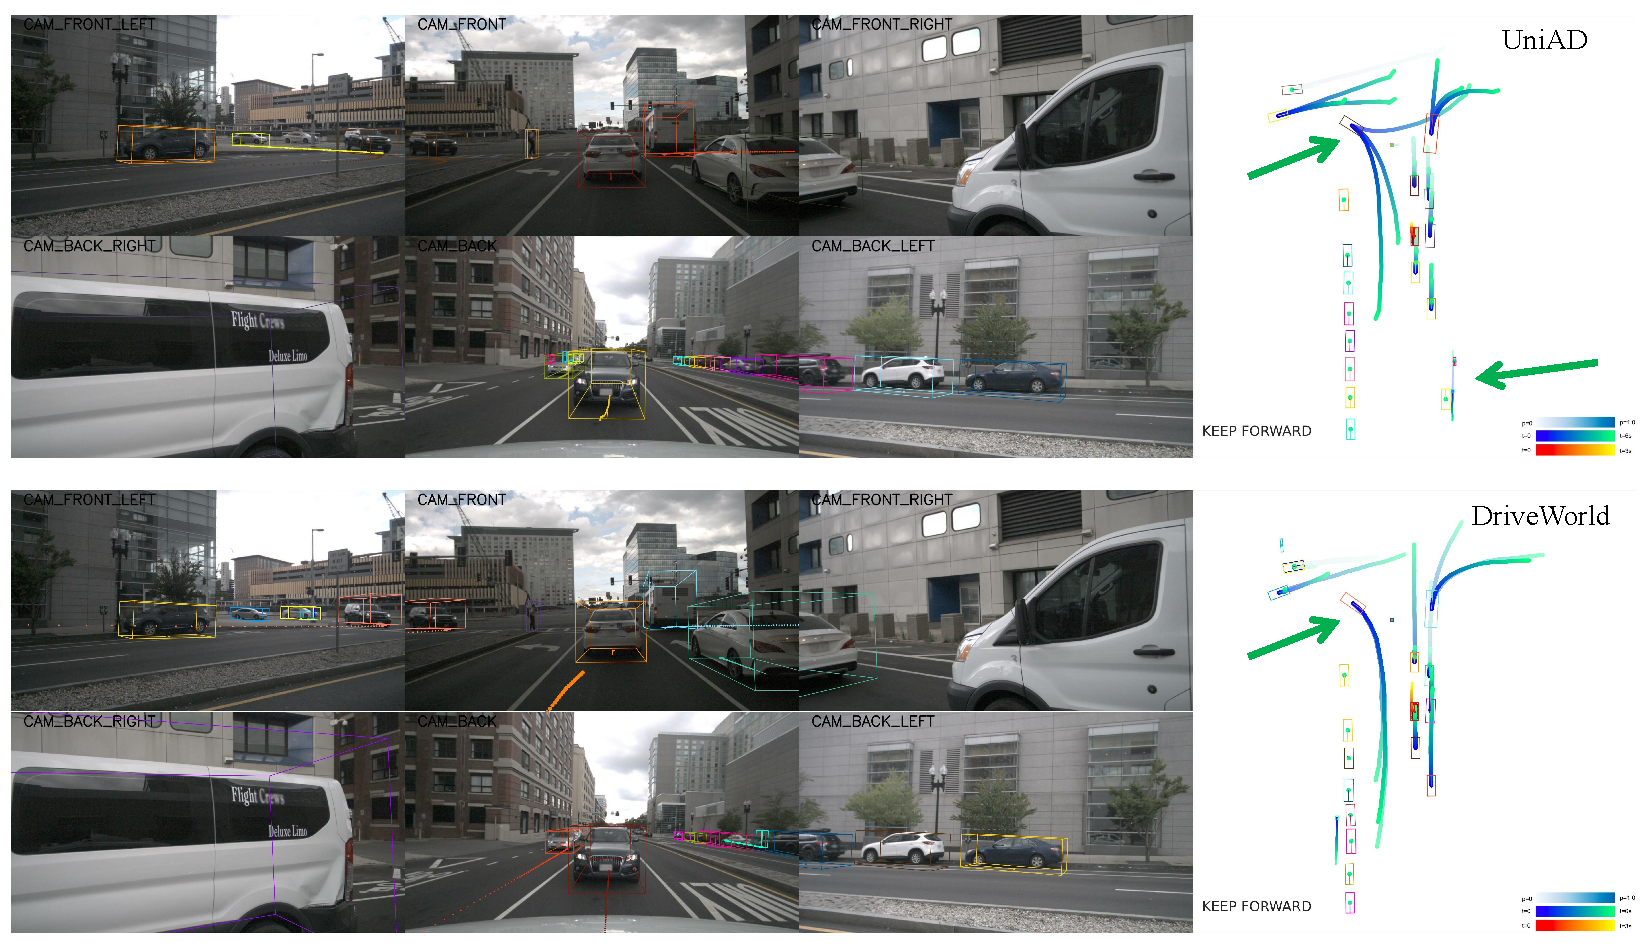
\includegraphics[width=0.5\textwidth]{figures/results} 
	\caption{Visual comparison between UniAD~\cite{uniad} (Top) and our DriveWorld (Bottom).}
	\label{fig:compare}
	%\vspace{-1em}
\end{figure}
We validate the performance on the online mapping task. As shown in Tab.~\ref{tab:mapping}, compared to UniAD, pre-training with 3D occupancy in OccNet and UniScene results in an improvement of about 1\% in IoU, and the knowledge distillation algorithm BEVDistill also enhances performance by 1\%. After our 4D pre-training on nuScenes, there is a 2\% improvement and a 3\% improvement after pre-training on OpenScene.
%\vspace{-1em}
\paragraph{Multi-object Tracking.}
We further evaluate the performance on the multi-object tracking task, which demands a deeper consideration of temporal information. Tab.~\ref{tab:mot} illustrates the outcomes of this evaluation. It is evident that leveraging DriveWorld's 4D pre-training results in a notable enhancement of 2.6\% in terms of AMOTA. Impressively, after pre-training on OpenScene, this performance boost becomes even more significant, reaching a substantial 5.3\% increase in AMOTA. In contrast, pre-training with OccNet, UniScene, and BEVDistill only provides a moderate improvement of 1.0\% in AMOTA. Furthermore, DriveWorld exhibits the lowest ID switch score, indicating that DriveWorld enables the model to consistently demonstrate temporal coherence for each tracklet.
%\vspace{-1em}
\paragraph{Motion Forecasting.}
In the motion prediction task, as demonstrated in Tab.~\ref{tab:forecasting}, the improvement obtained from 3D pre-training (\eg, OccNet, UniScene, and BEVDistill) is notably limited. In contrast, our 4D pre-training approach, which encompasses the capability to forecast future states, significantly enhances the performance of the motion prediction task. Pre-training on nuScenes results in a reduction of 0.04m in minADE, while pre-training on OpenScene leads to a remarkable 0.1m decrease in minADE. This notable improvement is partly attributed to the larger data scale of OpenScene and the presence of valuable flow information in this dataset. 
%\vspace{-1em}
\paragraph{Occupancy Prediction.}
The UniAD's occupancy prediction task is carried out in the 2D BEV view. As shown in Tab.~\ref{tab:occ}, after undergoing 4D occupancy pre-training on OpenScene, our model exhibits impressive enhancements: a 2.8\% increase in IoU-near, a 5\% boost in IoU-far, a 3.4\% gain in VPQ-near, and a 3.4\% rise in VPQ-far. This outcome underscores the effectiveness of our pre-training approach in achieving a more comprehensive reconstruction of 4D scenes.
%\vspace{-1em}
\paragraph{Planning.}
We finally validate the effectiveness of the proposed 4D pre-training algorithm on the planning task. As illustrated in Tab.~\ref{tab:planning}, DriveWorld stands out by achieving new state-of-the-art planning results, reducing an 0.34m average L2 error and an average Collision rate of 0.12. These results surpass the prior best model, UniAD. UniAD integrates perception, prediction, and planning in a sequential fashion. Our 4D pre-training approach, which comprehensively reconstructs the 3D scene, enhances tasks focused on the current scene, such as detection and segmentation. and predicts future scenarios elevating tracking and forecasting capabilities. By combining these advantages, we further improve the performance of the final planning step. Consequently, we have developed a robust fundamental model for autonomous driving. 

\subsection{Qualitative Results}
The qualitative comparison between UniAD and DriveWorld is visualized in Fig.~\ref{fig:compare}. UniAD exhibited false positives in detecting distant objects, and the detection accuracy was improved by DriveWorld. Additionally, UniAD made trajectory prediction errors for turning vehicles, which was addressed by DriveWorld after 4D pre-training, allowing for accurate predictions of future changes.
%The qualitative comparison depicted in Figure~\ref{fig:compare} highlights the distinctions between UniAD and DriveWorld. UniAD was observed to exhibit false positives particularly in the detection of distant objects, a limitation that DriveWorld notably addressed, leading to enhanced detection accuracy. Moreover, UniAD demonstrated trajectory prediction errors, especially concerning turning vehicles. However, DriveWorld, following 4D pre-training, effectively mitigated this issue, enabling precise predictions of future changes in trajectories.